% Created by tikzDevice version 0.12.6 on 2024-04-04 08:49:14
% !TEX encoding = UTF-8 Unicode
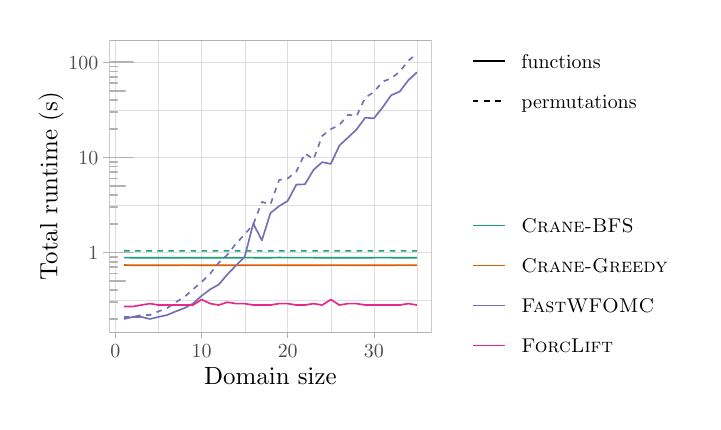
\begin{tikzpicture}[x=1pt,y=1pt]
\definecolor{fillColor}{RGB}{255,255,255}
\path[use as bounding box,fill=fillColor,fill opacity=0.00] (0,0) rectangle (240.29,135.16);
\begin{scope}
\path[clip] (  0.00,  0.00) rectangle (240.29,135.16);
\definecolor{drawColor}{RGB}{255,255,255}
\definecolor{fillColor}{RGB}{255,255,255}

\path[draw=drawColor,line width= 0.5pt,line join=round,line cap=round,fill=fillColor] (  0.00,  0.00) rectangle (240.29,135.16);
\end{scope}
\begin{scope}
\path[clip] ( 29.55, 25.11) rectangle (145.94,130.66);
\definecolor{fillColor}{RGB}{255,255,255}

\path[fill=fillColor] ( 29.55, 25.11) rectangle (145.94,130.66);
\definecolor{drawColor}{gray}{0.87}

\path[draw=drawColor,line width= 0.1pt,line join=round] ( 29.55, 36.74) --
	(145.94, 36.74);

\path[draw=drawColor,line width= 0.1pt,line join=round] ( 29.55, 71.11) --
	(145.94, 71.11);

\path[draw=drawColor,line width= 0.1pt,line join=round] ( 29.55,105.49) --
	(145.94,105.49);

\path[draw=drawColor,line width= 0.1pt,line join=round] ( 47.29, 25.11) --
	( 47.29,130.66);

\path[draw=drawColor,line width= 0.1pt,line join=round] ( 78.41, 25.11) --
	( 78.41,130.66);

\path[draw=drawColor,line width= 0.1pt,line join=round] (109.53, 25.11) --
	(109.53,130.66);

\path[draw=drawColor,line width= 0.1pt,line join=round] (140.65, 25.11) --
	(140.65,130.66);

\path[draw=drawColor,line width= 0.2pt,line join=round] ( 29.55, 53.93) --
	(145.94, 53.93);

\path[draw=drawColor,line width= 0.2pt,line join=round] ( 29.55, 88.30) --
	(145.94, 88.30);

\path[draw=drawColor,line width= 0.2pt,line join=round] ( 29.55,122.67) --
	(145.94,122.67);

\path[draw=drawColor,line width= 0.2pt,line join=round] ( 31.72, 25.11) --
	( 31.72,130.66);

\path[draw=drawColor,line width= 0.2pt,line join=round] ( 62.85, 25.11) --
	( 62.85,130.66);

\path[draw=drawColor,line width= 0.2pt,line join=round] ( 93.97, 25.11) --
	( 93.97,130.66);

\path[draw=drawColor,line width= 0.2pt,line join=round] (125.09, 25.11) --
	(125.09,130.66);
\definecolor{drawColor}{RGB}{27,158,119}

\path[draw=drawColor,line width= 0.6pt,line join=round] ( 34.84, 52.07) --
	( 37.95, 52.04) --
	( 41.06, 52.04) --
	( 44.17, 52.04) --
	( 47.29, 52.04) --
	( 50.40, 52.05) --
	( 53.51, 52.04) --
	( 56.62, 52.05) --
	( 59.73, 52.04) --
	( 62.85, 52.04) --
	( 65.96, 52.04) --
	( 69.07, 52.04) --
	( 72.18, 52.04) --
	( 75.30, 52.04) --
	( 78.41, 52.05) --
	( 81.52, 52.05) --
	( 84.63, 52.04) --
	( 87.74, 52.04) --
	( 90.86, 52.09) --
	( 93.97, 52.05) --
	( 97.08, 52.05) --
	(100.19, 52.05) --
	(103.31, 52.05) --
	(106.42, 52.04) --
	(109.53, 52.04) --
	(112.64, 52.04) --
	(115.75, 52.04) --
	(118.87, 52.04) --
	(121.98, 52.04) --
	(125.09, 52.05) --
	(128.20, 52.05) --
	(131.32, 52.05) --
	(134.43, 52.04) --
	(137.54, 52.05) --
	(140.65, 52.04);

\path[draw=drawColor,line width= 0.6pt,dash pattern=on 2pt off 2pt ,line join=round] ( 34.84, 54.53) --
	( 37.95, 54.50) --
	( 41.06, 54.50) --
	( 44.17, 54.49) --
	( 47.29, 54.49) --
	( 50.40, 54.49) --
	( 53.51, 54.49) --
	( 56.62, 54.50) --
	( 59.73, 54.50) --
	( 62.85, 54.49) --
	( 65.96, 54.49) --
	( 69.07, 54.49) --
	( 72.18, 54.49) --
	( 75.30, 54.49) --
	( 78.41, 54.50) --
	( 81.52, 54.50) --
	( 84.63, 54.50) --
	( 87.74, 54.50) --
	( 90.86, 54.49) --
	( 93.97, 54.50) --
	( 97.08, 54.50) --
	(100.19, 54.49) --
	(103.31, 54.50) --
	(106.42, 54.50) --
	(109.53, 54.50) --
	(112.64, 54.50) --
	(115.75, 54.49) --
	(118.87, 54.50) --
	(121.98, 54.50) --
	(125.09, 54.50) --
	(128.20, 54.50) --
	(131.32, 54.50) --
	(134.43, 54.50) --
	(137.54, 54.50) --
	(140.65, 54.50);
\definecolor{drawColor}{RGB}{217,95,2}

\path[draw=drawColor,line width= 0.6pt,line join=round] ( 34.84, 49.39) --
	( 37.95, 49.33) --
	( 41.06, 49.33) --
	( 44.17, 49.33) --
	( 47.29, 49.33) --
	( 50.40, 49.33) --
	( 53.51, 49.33) --
	( 56.62, 49.35) --
	( 59.73, 49.35) --
	( 62.85, 49.33) --
	( 65.96, 49.33) --
	( 69.07, 49.33) --
	( 72.18, 49.33) --
	( 75.30, 49.33) --
	( 78.41, 49.33) --
	( 81.52, 49.35) --
	( 84.63, 49.35) --
	( 87.74, 49.35) --
	( 90.86, 49.33) --
	( 93.97, 49.33) --
	( 97.08, 49.33) --
	(100.19, 49.33) --
	(103.31, 49.33) --
	(106.42, 49.33) --
	(109.53, 49.35) --
	(112.64, 49.35) --
	(115.75, 49.33) --
	(118.87, 49.33) --
	(121.98, 49.33) --
	(125.09, 49.33) --
	(128.20, 49.33) --
	(131.32, 49.33) --
	(134.43, 49.35) --
	(137.54, 49.35) --
	(140.65, 49.33);
\definecolor{drawColor}{RGB}{117,112,179}

\path[draw=drawColor,line width= 0.6pt,line join=round] ( 34.84, 29.90) --
	( 37.95, 30.63) --
	( 41.06, 30.63) --
	( 44.17, 29.90) --
	( 47.29, 30.63) --
	( 50.40, 31.33) --
	( 53.51, 32.63) --
	( 56.62, 33.82) --
	( 59.73, 35.45) --
	( 62.85, 38.26) --
	( 65.96, 40.62) --
	( 69.07, 42.34) --
	( 72.18, 46.05) --
	( 75.30, 49.23) --
	( 78.41, 52.36) --
	( 81.52, 64.35) --
	( 84.63, 58.30) --
	( 87.74, 68.19) --
	( 90.86, 70.67) --
	( 93.97, 72.59) --
	( 97.08, 78.45) --
	(100.19, 78.57) --
	(103.31, 83.81) --
	(106.42, 86.56) --
	(109.53, 85.94) --
	(112.64, 92.57) --
	(115.75, 95.46) --
	(118.87, 98.41) --
	(121.98,102.64) --
	(125.09,102.38) --
	(128.20,106.28) --
	(131.32,110.72) --
	(134.43,112.06) --
	(137.54,116.16) --
	(140.65,119.03);

\path[draw=drawColor,line width= 0.6pt,dash pattern=on 2pt off 2pt ,line join=round] ( 34.84, 30.63) --
	( 37.95, 30.63) --
	( 41.06, 31.33) --
	( 44.17, 31.33) --
	( 47.29, 32.63) --
	( 50.40, 33.82) --
	( 53.51, 35.96) --
	( 56.62, 37.83) --
	( 59.73, 40.62) --
	( 62.85, 43.28) --
	( 65.96, 46.30) --
	( 69.07, 50.22) --
	( 72.18, 53.16) --
	( 75.30, 57.14) --
	( 78.41, 60.47) --
	( 81.52, 64.05) --
	( 84.63, 72.20) --
	( 87.74, 71.34) --
	( 90.86, 80.12) --
	( 93.97, 80.67) --
	( 97.08, 83.21) --
	(100.19, 89.74) --
	(103.31, 87.61) --
	(106.42, 96.04) --
	(109.53, 98.47) --
	(112.64, 99.99) --
	(115.75,103.72) --
	(118.87,103.27) --
	(121.98,109.92) --
	(125.09,111.85) --
	(128.20,115.67) --
	(131.32,116.78) --
	(134.43,119.28) --
	(137.54,123.20) --
	(140.65,125.87);
\definecolor{drawColor}{RGB}{231,41,138}

\path[draw=drawColor,line width= 0.6pt,line join=round] ( 34.84, 34.38) --
	( 37.95, 34.38) --
	( 41.06, 34.93) --
	( 44.17, 35.45) --
	( 47.29, 34.93) --
	( 50.40, 34.93) --
	( 53.51, 34.93) --
	( 56.62, 34.93) --
	( 59.73, 34.93) --
	( 62.85, 36.92) --
	( 65.96, 35.45) --
	( 69.07, 34.93) --
	( 72.18, 35.96) --
	( 75.30, 35.45) --
	( 78.41, 35.45) --
	( 81.52, 34.93) --
	( 84.63, 34.93) --
	( 87.74, 34.93) --
	( 90.86, 35.45) --
	( 93.97, 35.45) --
	( 97.08, 34.93) --
	(100.19, 34.93) --
	(103.31, 35.45) --
	(106.42, 34.93) --
	(109.53, 36.92) --
	(112.64, 34.93) --
	(115.75, 35.45) --
	(118.87, 35.45) --
	(121.98, 34.93) --
	(125.09, 34.93) --
	(128.20, 34.93) --
	(131.32, 34.93) --
	(134.43, 34.93) --
	(137.54, 35.45) --
	(140.65, 34.93);
\definecolor{drawColor}{gray}{0.70}

\path[draw=drawColor,line width= 0.6pt,line join=round,line cap=round] ( 29.55, 29.90) -- ( 32.39, 29.90);

\path[draw=drawColor,line width= 0.6pt,line join=round,line cap=round] ( 29.55, 35.96) -- ( 32.39, 35.96);

\path[draw=drawColor,line width= 0.6pt,line join=round,line cap=round] ( 29.55, 40.25) -- ( 32.39, 40.25);

\path[draw=drawColor,line width= 0.6pt,line join=round,line cap=round] ( 29.55, 43.58) -- ( 35.24, 43.58);

\path[draw=drawColor,line width= 0.6pt,line join=round,line cap=round] ( 29.55, 46.30) -- ( 32.39, 46.30);

\path[draw=drawColor,line width= 0.6pt,line join=round,line cap=round] ( 29.55, 48.60) -- ( 32.39, 48.60);

\path[draw=drawColor,line width= 0.6pt,line join=round,line cap=round] ( 29.55, 50.60) -- ( 32.39, 50.60);

\path[draw=drawColor,line width= 0.6pt,line join=round,line cap=round] ( 29.55, 52.36) -- ( 32.39, 52.36);

\path[draw=drawColor,line width= 0.6pt,line join=round,line cap=round] ( 29.55, 53.93) -- ( 38.08, 53.93);

\path[draw=drawColor,line width= 0.6pt,line join=round,line cap=round] ( 29.55, 64.28) -- ( 32.39, 64.28);

\path[draw=drawColor,line width= 0.6pt,line join=round,line cap=round] ( 29.55, 70.33) -- ( 32.39, 70.33);

\path[draw=drawColor,line width= 0.6pt,line join=round,line cap=round] ( 29.55, 74.62) -- ( 32.39, 74.62);

\path[draw=drawColor,line width= 0.6pt,line join=round,line cap=round] ( 29.55, 77.95) -- ( 35.24, 77.95);

\path[draw=drawColor,line width= 0.6pt,line join=round,line cap=round] ( 29.55, 80.67) -- ( 32.39, 80.67);

\path[draw=drawColor,line width= 0.6pt,line join=round,line cap=round] ( 29.55, 82.98) -- ( 32.39, 82.98);

\path[draw=drawColor,line width= 0.6pt,line join=round,line cap=round] ( 29.55, 84.97) -- ( 32.39, 84.97);

\path[draw=drawColor,line width= 0.6pt,line join=round,line cap=round] ( 29.55, 86.73) -- ( 32.39, 86.73);

\path[draw=drawColor,line width= 0.6pt,line join=round,line cap=round] ( 29.55, 88.30) -- ( 38.08, 88.30);

\path[draw=drawColor,line width= 0.6pt,line join=round,line cap=round] ( 29.55, 98.65) -- ( 32.39, 98.65);

\path[draw=drawColor,line width= 0.6pt,line join=round,line cap=round] ( 29.55,104.70) -- ( 32.39,104.70);

\path[draw=drawColor,line width= 0.6pt,line join=round,line cap=round] ( 29.55,108.99) -- ( 32.39,108.99);

\path[draw=drawColor,line width= 0.6pt,line join=round,line cap=round] ( 29.55,112.32) -- ( 35.24,112.32);

\path[draw=drawColor,line width= 0.6pt,line join=round,line cap=round] ( 29.55,115.05) -- ( 32.39,115.05);

\path[draw=drawColor,line width= 0.6pt,line join=round,line cap=round] ( 29.55,117.35) -- ( 32.39,117.35);

\path[draw=drawColor,line width= 0.6pt,line join=round,line cap=round] ( 29.55,119.34) -- ( 32.39,119.34);

\path[draw=drawColor,line width= 0.6pt,line join=round,line cap=round] ( 29.55,121.10) -- ( 32.39,121.10);

\path[draw=drawColor,line width= 0.6pt,line join=round,line cap=round] ( 29.55,122.67) -- ( 38.08,122.67);

\path[draw=drawColor,line width= 0.5pt,line join=round,line cap=round] ( 29.55, 25.11) rectangle (145.94,130.66);
\end{scope}
\begin{scope}
\path[clip] (  0.00,  0.00) rectangle (240.29,135.16);
\definecolor{drawColor}{gray}{0.30}

\node[text=drawColor,anchor=base east,inner sep=0pt, outer sep=0pt, scale=  0.72] at ( 25.50, 51.45) {1};

\node[text=drawColor,anchor=base east,inner sep=0pt, outer sep=0pt, scale=  0.72] at ( 25.50, 85.82) {10};

\node[text=drawColor,anchor=base east,inner sep=0pt, outer sep=0pt, scale=  0.72] at ( 25.50,120.19) {100};
\end{scope}
\begin{scope}
\path[clip] (  0.00,  0.00) rectangle (240.29,135.16);
\definecolor{drawColor}{gray}{0.70}

\path[draw=drawColor,line width= 0.2pt,line join=round] ( 27.30, 53.93) --
	( 29.55, 53.93);

\path[draw=drawColor,line width= 0.2pt,line join=round] ( 27.30, 88.30) --
	( 29.55, 88.30);

\path[draw=drawColor,line width= 0.2pt,line join=round] ( 27.30,122.67) --
	( 29.55,122.67);
\end{scope}
\begin{scope}
\path[clip] (  0.00,  0.00) rectangle (240.29,135.16);
\definecolor{drawColor}{gray}{0.70}

\path[draw=drawColor,line width= 0.2pt,line join=round] ( 31.72, 22.86) --
	( 31.72, 25.11);

\path[draw=drawColor,line width= 0.2pt,line join=round] ( 62.85, 22.86) --
	( 62.85, 25.11);

\path[draw=drawColor,line width= 0.2pt,line join=round] ( 93.97, 22.86) --
	( 93.97, 25.11);

\path[draw=drawColor,line width= 0.2pt,line join=round] (125.09, 22.86) --
	(125.09, 25.11);
\end{scope}
\begin{scope}
\path[clip] (  0.00,  0.00) rectangle (240.29,135.16);
\definecolor{drawColor}{gray}{0.30}

\node[text=drawColor,anchor=base,inner sep=0pt, outer sep=0pt, scale=  0.72] at ( 31.72, 16.10) {0};

\node[text=drawColor,anchor=base,inner sep=0pt, outer sep=0pt, scale=  0.72] at ( 62.85, 16.10) {10};

\node[text=drawColor,anchor=base,inner sep=0pt, outer sep=0pt, scale=  0.72] at ( 93.97, 16.10) {20};

\node[text=drawColor,anchor=base,inner sep=0pt, outer sep=0pt, scale=  0.72] at (125.09, 16.10) {30};
\end{scope}
\begin{scope}
\path[clip] (  0.00,  0.00) rectangle (240.29,135.16);
\definecolor{drawColor}{RGB}{0,0,0}

\node[text=drawColor,anchor=base,inner sep=0pt, outer sep=0pt, scale=  0.90] at ( 87.74,  6.25) {Domain size};
\end{scope}
\begin{scope}
\path[clip] (  0.00,  0.00) rectangle (240.29,135.16);
\definecolor{drawColor}{RGB}{0,0,0}

\node[text=drawColor,rotate= 90.00,anchor=base,inner sep=0pt, outer sep=0pt, scale=  0.90] at ( 10.70, 77.89) {Total runtime (s)};
\end{scope}
\begin{scope}
\path[clip] (  0.00,  0.00) rectangle (240.29,135.16);
\definecolor{fillColor}{RGB}{255,255,255}

\path[fill=fillColor] (154.94, 96.84) rectangle (224.55,147.20);
\end{scope}
\begin{scope}
\path[clip] (  0.00,  0.00) rectangle (240.29,135.16);
\definecolor{fillColor}{RGB}{255,255,255}

\path[fill=fillColor] (159.44,115.79) rectangle (173.90,130.25);
\end{scope}
\begin{scope}
\path[clip] (  0.00,  0.00) rectangle (240.29,135.16);
\definecolor{drawColor}{RGB}{0,0,0}

\path[draw=drawColor,line width= 0.6pt,line join=round] (160.89,123.02) -- (172.45,123.02);
\end{scope}
\begin{scope}
\path[clip] (  0.00,  0.00) rectangle (240.29,135.16);
\definecolor{fillColor}{RGB}{255,255,255}

\path[fill=fillColor] (159.44,101.34) rectangle (173.90,115.79);
\end{scope}
\begin{scope}
\path[clip] (  0.00,  0.00) rectangle (240.29,135.16);
\definecolor{drawColor}{RGB}{0,0,0}

\path[draw=drawColor,line width= 0.6pt,dash pattern=on 2pt off 2pt ,line join=round] (160.89,108.57) -- (172.45,108.57);
\end{scope}
\begin{scope}
\path[clip] (  0.00,  0.00) rectangle (240.29,135.16);
\definecolor{drawColor}{RGB}{0,0,0}

\node[text=drawColor,anchor=base west,inner sep=0pt, outer sep=0pt, scale=  0.72] at (178.40,120.54) {functions};
\end{scope}
\begin{scope}
\path[clip] (  0.00,  0.00) rectangle (240.29,135.16);
\definecolor{drawColor}{RGB}{0,0,0}

\node[text=drawColor,anchor=base west,inner sep=0pt, outer sep=0pt, scale=  0.72] at (178.40,106.09) {permutations};
\end{scope}
\begin{scope}
\path[clip] (  0.00,  0.00) rectangle (240.29,135.16);
\definecolor{fillColor}{RGB}{255,255,255}

\path[fill=fillColor] (154.94,  8.58) rectangle (235.79, 87.84);
\end{scope}
\begin{scope}
\path[clip] (  0.00,  0.00) rectangle (240.29,135.16);
\definecolor{fillColor}{RGB}{255,255,255}

\path[fill=fillColor] (159.44, 56.44) rectangle (173.90, 70.89);
\end{scope}
\begin{scope}
\path[clip] (  0.00,  0.00) rectangle (240.29,135.16);
\definecolor{drawColor}{RGB}{27,158,119}

\path[draw=drawColor,line width= 0.6pt,line join=round] (160.89, 63.66) -- (172.45, 63.66);
\end{scope}
\begin{scope}
\path[clip] (  0.00,  0.00) rectangle (240.29,135.16);
\definecolor{fillColor}{RGB}{255,255,255}

\path[fill=fillColor] (159.44, 41.98) rectangle (173.90, 56.44);
\end{scope}
\begin{scope}
\path[clip] (  0.00,  0.00) rectangle (240.29,135.16);
\definecolor{drawColor}{RGB}{217,95,2}

\path[draw=drawColor,line width= 0.6pt,line join=round] (160.89, 49.21) -- (172.45, 49.21);
\end{scope}
\begin{scope}
\path[clip] (  0.00,  0.00) rectangle (240.29,135.16);
\definecolor{fillColor}{RGB}{255,255,255}

\path[fill=fillColor] (159.44, 27.53) rectangle (173.90, 41.98);
\end{scope}
\begin{scope}
\path[clip] (  0.00,  0.00) rectangle (240.29,135.16);
\definecolor{drawColor}{RGB}{117,112,179}

\path[draw=drawColor,line width= 0.6pt,line join=round] (160.89, 34.76) -- (172.45, 34.76);
\end{scope}
\begin{scope}
\path[clip] (  0.00,  0.00) rectangle (240.29,135.16);
\definecolor{fillColor}{RGB}{255,255,255}

\path[fill=fillColor] (159.44, 13.08) rectangle (173.90, 27.53);
\end{scope}
\begin{scope}
\path[clip] (  0.00,  0.00) rectangle (240.29,135.16);
\definecolor{drawColor}{RGB}{231,41,138}

\path[draw=drawColor,line width= 0.6pt,line join=round] (160.89, 20.30) -- (172.45, 20.30);
\end{scope}
\begin{scope}
\path[clip] (  0.00,  0.00) rectangle (240.29,135.16);
\definecolor{drawColor}{RGB}{0,0,0}

\node[text=drawColor,anchor=base west,inner sep=0pt, outer sep=0pt, scale=  0.72] at (178.40, 61.18) {\textsc{Crane-BFS}};
\end{scope}
\begin{scope}
\path[clip] (  0.00,  0.00) rectangle (240.29,135.16);
\definecolor{drawColor}{RGB}{0,0,0}

\node[text=drawColor,anchor=base west,inner sep=0pt, outer sep=0pt, scale=  0.72] at (178.40, 46.73) {\textsc{Crane-Greedy}};
\end{scope}
\begin{scope}
\path[clip] (  0.00,  0.00) rectangle (240.29,135.16);
\definecolor{drawColor}{RGB}{0,0,0}

\node[text=drawColor,anchor=base west,inner sep=0pt, outer sep=0pt, scale=  0.72] at (178.40, 32.28) {\textsc{FastWFOMC}};
\end{scope}
\begin{scope}
\path[clip] (  0.00,  0.00) rectangle (240.29,135.16);
\definecolor{drawColor}{RGB}{0,0,0}

\node[text=drawColor,anchor=base west,inner sep=0pt, outer sep=0pt, scale=  0.72] at (178.40, 17.82) {\textsc{ForcLift}};
\end{scope}
\end{tikzpicture}
